\documentclass[UTF8]{ctexart}
\usepackage{amsmath}
\usepackage{graphicx}
\usepackage{float}
\usepackage{subfigure}
\usepackage{xeCJK}
\usepackage{hyperref}
\usepackage{algorithm2e}
\usepackage{amsfonts}
\usepackage{epsfig}
\usepackage{listings}
\usepackage{xcolor}
% 定义可能使用到的颜色

\definecolor{CPPLight}  {HTML} {686868}
\definecolor{CPPSteel}  {HTML} {888888}
\definecolor{CPPDark}   {HTML} {262626}
\definecolor{CPPBlue}   {HTML} {4172A3}
\definecolor{CPPGreen}  {HTML} {487818}
\definecolor{CPPBrown}  {HTML} {A07040}
\definecolor{CPPRed}    {HTML} {AD4D3A}
\definecolor{CPPViolet} {HTML} {7040A0}
\definecolor{CPPGray}  {HTML} {B8B8B8}
\lstset{
    columns=fixed,
    numbers=left,                                        % 在左侧显示行号
    frame=none,                                          % 不显示背景边框
    backgroundcolor=\color[RGB]{245,245,244},            % 设定背景颜色
    keywordstyle=\color[RGB]{40,40,255},                 % 设定关键字颜色
    numberstyle=\footnotesize\color{darkgray},           % 设定行号格式
    commentstyle=\it\color[RGB]{0,96,96},                % 设置代码注释的格式
    stringstyle=\rmfamily\slshape\color[RGB]{128,0,0},   % 设置字符串格式
    showstringspaces=false,                              % 不显示字符串中的空格
    language=c++,                                        % 设置语言
    morekeywords={alignas,continute,friend,register,true,alignof,decltype,goto,
    reinterpret_cast,try,asm,defult,if,return,typedef,auto,delete,inline,short,
    typeid,bool,do,int,signed,typename,break,double,long,sizeof,union,case,
    dynamic_cast,mutable,static,unsigned,catch,else,namespace,static_assert,using,
    char,enum,new,static_cast,virtual,char16_t,char32_t,explict,noexcept,struct,
    void,export,nullptr,switch,volatile,class,extern,operator,template,wchar_t,
    const,false,private,this,while,constexpr,float,protected,thread_local,
    const_cast,for,public,throw,std},
}

\graphicspath{{images/}}
\setCJKmonofont{Microsoft YaHei}

\title{\Huge{计算机算法设计与分析\\ 动态规划}}
\author{\Huge{易凯}}
\date{\Huge{2017年4月18日}}

\begin{document}
    \maketitle
    \vspace{35mm}
    \begin{flushright}
    \Large{
    \textbf{班\ \ \ \ \ 级} \makebox[5em][l]{软件53班}

    \textbf{学\ \ \ \ \ 号} \makebox[5em][l]{2151601053}

    \textbf{邮\ \ \ \ \ 箱} \makebox[5em][l]{williamyi96@gmail.com}

    \textbf{联系电话} \makebox[5em][l]{13772103675}

    \textbf{个人网站} \makebox[5em][l]{https://williamyi96.github.io}

                      \makebox[5em][l]{williamyi.tech}

      \textbf{实验日期} \makebox[5em][l]{2017年4月18日}

    \textbf{提交日期} \makebox[5em][l]{2017年6月6日}
    }
    \end{flushright}
    
    \newpage
  	\tableofcontents
  	\newpage
  	\listoffigures
    \newpage
    
    \section{基本声明}
    此动态规划的相关作业,是在完成《计算机算法设计与分析》的布置习题的基础上,对于《算法导论》对应章节的课后题的程序实现。

    \section{DP问题的基本方法}
    \subsection{DP概念}
    动态规划方法通常用于求解最优化问题。这类问题往往有很多个解,但是我们需要找到这些解中的最优解(最优解就是最大值或者最小值的解)。

    动态规划方法与分治法最大的差别是,分治法的子问题之间相互没有包含关系,而动态规划方法的子问题则存在着包含关系,分治法的求解会反复地求解公共子问题,而动态规划方法采用制表待查的方式使公共子问题只需要计算一次。从而将许多需要指数级时间才能够计算完成的算法只需要平方级别或者立方级别就可以完成。

    \subsection{动态规划算法的实现步骤}
    1. 刻画一个最优解的结构特征;

    2. 递归地定义最优解的值;

    3. 计算最优解的值,通常采用自底向上的方法

    4. 利用计算出的信息构造一个最优解

    \section{最长单调递增子序列}
    \subsection{题目描述}
    设计一个$O(n^2)$ 时间的算法,找出由n个数组成的序列的最长单调递增子序列。

    \subsection{试题分析}
    我们可以使用数组b[0:n-1]记录a[i], 0<=i<=n, 为结尾元素的最长递增子序列的长度。序列a的最长递增子序列的长度为max{b[i]}。

    首先,b[i]满足最优子结构,因为如果a[i]不是b[j]的最长单调递增子序列,而a[k]是其的最长单调递增子序列,那么用a[k]替换为a[i]即可,则最后b[i]为最优子结构。

    因此我们可以递归地定义最优解的值:
    b[0] = 1, b[i] = max{b[k]} + 1

    \subsection{算法实现}
    \paragraph{Java实现}

\begin{small}
\begin{lstlisting}[language=java]
package lis;

import java.util.Scanner;

public class LIS_DP {
	//dp[i]记录[0:i]数组的LIS,lis表示LIS的长度
	static int[] dp = new int[100];
	static int lis;
	
	static int LIS_dp(int arr[], int size) {
		for(int i = 0; i < size; i++) {
			dp[i] = 1;
			for(int j = 0; j < i; j++) {
				if(arr[i] > arr[j] && dp[i] < dp[j] + 1) {
					dp[i] = dp[j] + 1;
					if(dp[i] > lis) lis = dp[i];
				}
			}
		}
		return lis;
	}
	
	static void outputLIS(int arr[], int index) {
		boolean isLIS = false;
		if(index < 0 || lis == 0) return;
		if(dp[index] == lis) {lis--; isLIS= true;}
		if(isLIS) System.out.println(arr[index+1]);
	}
	
	public static void main(String[] args) {
		//int [] arr = new int[100];
		int arr[] = {1,2,3,5,4,9,8,7};
//		如何设置任意输出的字符串向整数的转化
//		Scanner sc = new Scanner(System.in);		
//		System.out.println("Please input the array");
//		for(sc.nextInt()) {
//			arr = sc.nextInt();
//		}
		System.out.println(LIS_dp(arr, arr.length));
		
		outputLIS(arr, (arr.length - 1));
		System.out.println();
	}
}
\end{lstlisting}
\end{small}

    \paragraph{Cpp实现}

\begin{small}
\begin{lstlisting}[language=c++]
#include <iostream>
using namespace std;

/* 最长递增子序列 LIS
 * 设数组长度不超过 30
 * DP
*/

int dp[31]; /* dp[i]记录到[0,i]数组的LIS */
int lis;    /* LIS 长度 */

int LIS(int * arr, int size){
    for(int i = 0; i < size; ++i){
        dp[i] = 1;
        for(int j = 0; j < i; ++j){
            if(arr[i] > arr[j] && dp[i] < dp[j] + 1){
                dp[i] = dp[j] + 1;
                if(dp[i] > lis) lis = dp[i];
            }
        }
    }
    return lis;
}

/* 输出LIS */
void outputLIS(int * arr, int index) {
    bool isLIS = 0;
    if(index < 0 || lis == 0) return;

    if(dp[index] == lis) {--lis; isLIS = 1;}

    outputLIS(arr,--index);

    if(isLIS) printf("%d ",arr[index+1]);
}

int main() {
    int arr[] = {1,-1,2,-3,4,-5,6,-7};

    /* 输出LIS长度; sizeof 计算数组长度 */
    printf("%d\n",LIS(arr,sizeof(arr)/sizeof(int)));

    /* 输出LIS */
    outputLIS(arr,sizeof(arr)/sizeof(int) - 1);
    printf("\n");
}
\end{lstlisting}
\end{small}

    在使用java进行代码实现时,只能够输出LIS,但是不能够输出LIS具体内容,遇到这样的问题如何进行处理?继续深入研究!

    \section{编辑距离问题}
    \subsection{问题描述}
    设A和B是两个字符串。要用最少的字符操作将字符串A转换为字符串B。这里所说的字符操作包括:1).删除一个字符;2).插入一个字符;3)将一个字符改为另一个字符。

    将字符串A变换为字符串B所用的最少字符操作数称为字符串A到B的编辑距离,记为d(A,B)。试设计一个有效算法,对任给的两个字符串A和B,计算出他们的编辑距离d(A,B)。

    也就是对于给定的字符串A和B,计算其编辑距离d(A,B).

    \subsection{数据输入与结果输出}
    \paragraph{数据输入}
    文件的第一行是字符串A,文件的第二行是字符串B。

    \paragraph{结果输出}
    将编辑距离d(A,B)直接输出。

    \subsection{算法分析与设计}
    此题为使用动态规划的基础之上,然后利用相关vector完成基本的操作。值得注意的是,有效地字符操作数只有三种。

    \subsection{代码实现}
    \begin{small}
    \begin{lstlisting}
    #include <stdio.h>
#include <string.h>
using namespace std;

char s1[1000],s2[1000];

int min(int a,int b,int c) {
    int t = a < b ? a : b;
    return t < c ? t : c;
}
void editDistance(int len1,int len2) {
    int** d=new int*[len1+1];
    for(int k=0;k<=len1;k++)
        d[k]=new int[len2+1];
    int i,j;
    for(i = 0;i <= len1;i++)
        d[i][0] = i;
    for(j = 0;j <= len2;j++)
        d[0][j] = j;
    for(i = 1;i <= len1;i++)
        for(j = 1;j <= len2;j++) {
            int cost = s1[i] == s2[j] ? 0 : 1;
            int deletion = d[i-1][j] + 1;
            int insertion = d[i][j-1] + 1;
            int substitution = d[i-1][j-1] + cost;
            d[i][j] = min(deletion,insertion,substitution);
        }
    printf("%d\n",d[len1][len2]);
    for(int k=0;i<=len1;k++)
        delete[] d[k];
    delete[] d;
}
int main() {
    while(scanf("%s %s",s1,s2) != EOF)
        editDistance(strlen(s1),strlen(s2));
}
    \end{lstlisting}
    \end{small}

    \subsection{运行结果}
    \begin{figure}[!htb]
      \centering
      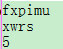
\includegraphics[width=0.3\textwidth]{../img/2.PNG}
      \caption{编辑距离问题运行示例}\label{编辑距离问题运行示例}
    \end{figure}

    \section{数字三角形问题}
    \subsection{问题描述}
    给定一个由n行数字组成的数字三角形。试设计一种算法,计算出从三角形的顶到底的一条路径,使该路径经过的数字总和最大。

    \subsection{数据输入与结果输出}
    \paragraph{数据输入}
    文件的第一行是数字三角形的行数,接下来的n行是数字三角形各行中的数字。所有数字都在0-99之间。

    \paragraph{结果输出}
    将计算结果输出中的第一行就表示所得到的计算出的最大值。

    \subsection{算法分析与设计}
    该问题只需要在三角形的每一层中选择最大的数字,然后构成一条路径即可。

    \subsection{代码实现}
\begin{small}
\begin{lstlisting}[language=java]
package maxtriangle;

public class MaxTriangle {
	
	static int maxTriangle(int mat[][], int row, int col) {
		int max = 0, sum = 0;
		if(row == 0) return sum;
		for(int k = 0; k < col; k++) {
			if(mat[row][k] > max) max = mat[row][k];
			sum += maxTriangle(mat, row-1, col-1);
		}
		return sum;
	}
	
	public static void main(String[] args) {
		int[][] mat= {{7,},{3,8},{8,1,0},{2,7,4,4},{4,5,2,6,5}};
		System.out.println(maxTriangle(mat, 5, 5));
		
	}
}
\end{lstlisting}
\end{small}

    \subsection{反思总结}
    相比较而言,此动态规划问题较为简单,思考如果按照上述格式完成有可能不会得到预期结果的根本原因。

    \section{汽车加油行驶问题}
    \subsection{问题描述}
    给定一个N*N的网格,设其左上角为起点,坐标为(1,1), X轴向右为正,Y轴向下为正,每个方格边长为1.一辆汽车从起点驶向终点,其坐标为(N,N)。如果在若干网格的交叉点处,设置了油库,可供汽车在行驶途中加油。汽车在行驶过程中应该遵守如下规则:

    1. 汽车只能够沿着网格行驶,装满油后汽车能够行驶K条网格边。出发时汽车已经装满油,在起点和终点处不设油库。

    2. 当汽车行驶经过一条网格边时,若其X坐标或者Y坐标减小,则应付费用B,否则免付费用。

    3. 汽车在行驶过程中遇油库则应该加满油并支付加油费用A。

    4. 在需要时可在网格点处增设油库,并付增设油库费用C(不含加油费用A)。

    5. 其中上述四步的所有数均为正整数。

    \subsection{算法设计}
    求汽车从起点出发到终点的一条所付费用最少的行驶路线。

    \subsection{输入与输出}

    输入为每个一组NKABC正整数,然后接着N行的加油点情况(0表示没有,1表示有)。

    输出是支付费用最少的路线。

    \subsection{算法分析}
    此题为典型的使用动态规划求解的例子,当全局的费用最少时,也就是达到全局最优时,那么局部一定是最优的。

    \subsection{程序实现}
    \begin{small}
    \begin{lstlisting}[language=c++]
#include <cstdio>
#include <queue>
#include <cstring>
#include <algorithm>
#define N 105
#define K 15
#define inf 0x3f3f3f3f
using namespace std;
const int dx[4]={1,0,-1,0};
const int dy[4]={0,1,0,-1};
struct Lux
{
    int k,x,y;
    Lux(int a,int b,int c):k(a),x(b),y(c){}
    Lux(){}
};

int map[N][N],id[N][N],cnt;
int n,p,A,B,C;
int dist[K][N][N];
bool in[K][N][N];
Lux s,t;

int spfa()  {
    int i,vx,vy,fee,fee2;
    queue<Lux>q;
    memset(dist,0x3f,sizeof(dist));
    dist[s.k][s.x][s.y]=0;
    in[s.k][s.x][s.y]=1;
    q.push(s);
    while(!q.empty())
    {
        Lux U=q.front();q.pop();in[U.k][U.x][U.y]=0;
        if(!U.k)continue;
        for(fee=i=0;i<4;i++)  {
            vx=U.x+dx[i];
            vy=U.y+dy[i];
            if(i==2)fee=B;/*往回走要多付的费用在这里处理。*/
            if(!id[vx][vy])continue;
            if(!map[vx][vy])
            {
                fee2=C;/*新开油站,准确的说这里的思想是把全图都开成加油站,原加油站强制加油,新加油站不强制,但加油要多付钱*/
                if(U.k&&dist[U.k-1][vx][vy]>dist[U.k][U.x][U.y]+fee)
                {/*因为加油站强制加油,所以不是加油站才能这么转移。*/
                    dist[U.k-1][vx][vy]=dist[U.k][U.x][U.y]+fee;
                    if(!in[U.k-1][vx][vy])in[U.k-1][vx][vy]=1,q.push(Lux(U.k-1,vx,vy));
                }
            }
            else fee2=0;/*已经有原加油站了就不需要再付额外费用了*/

            if(dist[p][vx][vy]>dist[U.k][U.x][U.y]+A+fee+fee2)
            {/*加油的转移*/
                dist[p][vx][vy]=dist[U.k][U.x][U.y]+A+fee+fee2;
                if(!in[p][vx][vy])in[p][vx][vy]=1,q.push(Lux(p,vx,vy));
            }
        }
    }
    int ret=inf;
    for(i=0;i<=p;i++)ret=min(ret,dist[i][t.x][t.y]);
    return ret;
}

int main()  {
    scanf("%d%d%d%d%d",&n,&p,&A,&B,&C);
    for(int i=1;i<=n;i++)for(int j=1;j<=n;j++)scanf("%d",&map[i][j]),id[i][j]=++cnt;
    s=Lux(p,1,1),t=Lux(0,n,n);
    printf("%d\n",spfa());
    return 0;
}
    \end{lstlisting}
    \end{small}

    \subsection{结果示例}
    \begin{figure}[!htb]
      \centering
      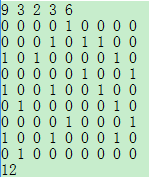
\includegraphics[width=0.6\textwidth]{../img/1.PNG}
      \caption{汽车加油行驶问题示例运行}\label{汽车加油行驶问题示例运行}
    \end{figure}

    \section{最少费用购物问题}
    \subsection{习题描述}
    某商店中每种商品都有一个价格。例如,一朵花的价格是2元;一个花瓶的价格是5元。为了吸引更多的顾客,商店提供了特殊优惠价。

    特殊优惠商品是把一种或几种商品分成一组。并降价销售。例如:3朵花的价格不是6而是5元;2个花瓶加1朵花是10 ICU不是12元。

    编一个程序,计算某个顾客所购商品应付的费用。要充分利用优惠价以使顾客付款最小。请注意,你不能变更顾客所购商品的种类及数量,即使增加某些商品会使付款总数减小也不允许你作出任何变更。假定各种商品价格用优惠价如上所述,并且某顾客购买物品为:3朵花和2个花瓶。那么顾客应付款为14元因为:

    1朵花加2个花瓶: 优惠价:10元; 2朵花  ,正常价:4元

    \subsection{算法设计}
    对于给定预购商品的价格和数量,以及优惠商品价,计算所购商品应付的最少费用。

    \subsection{数据输入}
    用两个文件表示输入数据。第一个文件INPUT.TXT描述顾客所购物品(放在购物筐中);第二个文件描述商店提供的优惠商品及价格(文件名为OFFER.TXT)。 两个文件中都只用整数。

    第一个文件INPUT.TXT的格式为:第一行是一个数字B(0≤B≤5),表示所购商品种类数。下面共B行,每行中含3个数C,K,P。C 代表商品的编码(每种商品有一个唯一的编码),1≤C≤999。K代表该种商品购买总数,1≤K≤5。P 是该种商品的正常单价(每件商品的价格),1≤P≤999。请注意,购物筐中最多可放5*5=25件商品。

    第二个文件OFFER.TXT的格式为:第一行是一个数字S(0≤S≤99),表示共有S种优惠。下面共S行,每一行描述一种优惠商品的组合中商品的种类。下面接着是几个数字对(C,K),其中C代表商品编码,1≤C≤9 99。K代表该种商品在此组合中的数量,1≤K≤5。本行最后一个数字P(1≤P≤9999)代表此商品组合的优惠价。当然, 优惠价要低于该组合中商品正常价之总和。

    \subsection{数据输出}
    将计算出的所购商品应付的最少费用输出到文件OUTPUT.TXT。

    \subsection{分析}
    通过动态规划进行求解,我们可以得到状态转移方程:
    F [a, b, c, d, e] = Min {F [a-S1, b-S2, c-S3, d-S4, e-S5] + SaleCost [S]}

    初始条件为:F [a, b, c, d, e] = Cost [1]*a+Cost [2]*b+Cost [3]*c+Cost [4]*d+Cost [5]*e。 即不用优惠的购买费用。

    \subsection{代码实现}
    \begin{small}
    \begin{lstlisting}
    #include <iostream>
#include <cstdio>
#include <algorithm>
#include <cstring>
#include <queue>
#include <set>
#include <map>
#include <time.h>
using namespace std;

int sale[1000][6] = {0};    //分别表示每个优惠中每个商品数量
int saleprice[1000] = {0};  //优惠总价
int salelength[1000] = {0}; //优惠总共有几个商品
int salenumber[1000][1000] = {0};   //优惠商品的ID
int good[6][4] = {0};       //1 -> number   2 -> price  3 -> last num
int num[1000];              //商品ID
int dp[6][6][6][6][6];
int n,m;

void input()  {
        cin>>n;
        for(int i = 1; i  <= n; i++)  {
            cin>>good[i][1]>>good[i][3]>>good[i][2];
            num[i] = good[i][1];
        }
        cin>>m;
        for(int i = 1; i <= m; i++)  {
                cin>>salelength[i];
                for(int j = 1; j <= salelength[i]; j++)  {
                        cin>>salenumber[i][j];
                        cin>>sale[i][salenumber[i][j]];
                }
                cin>>saleprice[i];
        }
}

void output()  {
    for(int i = 1; i  <= n; i++)
        cout<<"goodnum: "<<good[i][1]<<" goodprice: "
			<<good[i][2]<<" goodlast: "<<good[i][3]<<endl;
    for(int i = 1; i  <= m; i++)  {
        cout<<"sale"<<i<<" : ";
        for(int j = 1; j <= salelength[i]; j++)
                cout<<"num: "<<salenumber[i][j]<<"
                count: "<<sale[i][salenumber[i][j]]<<" ";
        cout<<endl;
        cout<<" price: "<<saleprice[i]<<endl;
    }
}

int main()  {
    //freopen("in2","r",stdin);
    input();
    // output();
    dp[0][0][0][0][0] = 0;
    for(int i = 0; i <= good[1][3]; i++)
        for(int j= 0; j <= good[2][3]; j++)
            for(int k = 0; k <= good[3][3] ;k++)
                for(int l = 0; l <= good[4][3]; l++)
                    for(int p = 0; p <= good[5][3]; p++) {
	int minx = i * good[1][2] + j
         * good[2][2] + k * good[3][2]
	 	 + l * good[4][2] + p * good[5][2];
	for(int q = 1; q <= m; q++)  {
	  if(i -sale[q][num[1]]<0 || i - sale[q][num[2]]<0 ||
		    i-sale[q][num[3]]<0 || i-sale[q][num[4]]<0 ||
            i-sale[q][num[5]]<0)  continue;
	   int t = dp[i - sale[q][num[1]]][j -
            sale[q][num[2]]][k - sale[q][num[3]]]
			[l - sale[q][num[4]]][p - sale[q][num[5]]] + saleprice[q];
	   if(t < minx) minx = t;
	   }
		dp[i][j][k][l][p] = minx;
	}
    cout<<dp[good[1][3]][good[2][3]]
        [good[3][3]][good[4][3]][good[5][3]]<<endl;
	return 0;
}
    \end{lstlisting}
    \end{small}

    \subsection{样例测试}
    \begin{figure}[!htb]
      \centering
      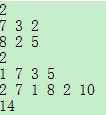
\includegraphics[width=0.5\textwidth]{../img/3.PNG}
      \caption{最少购物费用问题示例运行}\label{最少购物费问题示例运行}
    \end{figure}

    \section{收集样本问题}
    \subsection{习题描述}
    机器人在一个正方形方格之内收集样本。试找出两条行走路径,使其取得的样本总价值最大。

    \subsection{算法设计}
    给定方形区域F的样本分布,计算Rob的两条行走路径,使其取得的样本总价值最大。

    \subsection{数据输入}
    首先输入矩阵的规模,然后在输入样本所在的位置以及价值。

    \subsection{数据输出}
    计算得到的最大的样本总价值。

    \subsection{代码实现}
    \begin{small}
    \begin{lstlisting}
#include <iostream>
#include <cstdio>
#include <string.h>
using namespace std;

#define MAXN 22

int h[MAXN][MAXN][MAXN][MAXN];
int v[MAXN][MAXN];
int n;

void update(int x1, int y1, int x2, int y2, int val) {
	if(y1 >= n || y2 >= n) return;
	if(x1 >= n || x2 >= n) return;
	if(x1 == x2 && y1 == y2) {
		h[x1][y1][x2][y2] = max(h[x1][y1][x2][y2],
			val + v[x1][y1]);
	} else {
		h[x1][y1][x2][y2] = max(h[x1][y1][x2][y2],
			val + v[x1][y1] + v[x2][y2]);
	}
}

int main() {
	scanf("%d", &n);
	memset(v, 0, sizeof(v));
	int x, y, val;
	while(scanf("%d %d %d", &x, &y, &val) && x != 0) {
		v[x - 1][y - 1] = val;
	}
	memset(h, 0, sizeof(h));
	h[0][0][0][0] = v[0][0];

	for(int s = 0; s < 2 * n - 2; ++s) {
		for(int x1 = 0; x1 < n && x1 <= s; ++x1) {
			for(int x2 = 0; x2 < n && x2 <= s; ++x2) {
			int y1 = s - x1;
			int y2 = s - x2;
			int v = h[x1][y1][x2][y2];

			update(x1 + 1, y1, x2 + 1, y2, v);
			update(x1 + 1, y1, x2, y2 + 1, v);
			update(x1, y1 + 1, x2 + 1, y2, v);
			update(x1, y1 + 1, x2, y2 + 1, v);
			}
		}
	}
	printf("%d\n", h[n - 1][n - 1][n - 1][n - 1]);
	return 0;
}
    \end{lstlisting}
    \end{small}

    \subsection{样例测试}
    \begin{figure}[!htb]
      \centering
      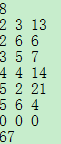
\includegraphics[width=0.3\textwidth]{../img/4.PNG}
      \caption{机器人收集样本问题示例运行}\label{机器人收集样本问题示例运行}
    \end{figure}

    \section{参考资料}
    1. LIS.http://www.ahathinking.com/archives/117.html

    2. Thomas H.Cormen, Charles E.Leiserson, Ronald L.Rivest, Clifford Stein. Introduction to Algorithms.

\end{document} 